\documentclass[10pt]{article}
\usepackage[a4paper,margin=18mm]{geometry}
\usepackage{amsmath,amssymb,booktabs,array,enumitem}
\usepackage[T1]{fontenc}\usepackage{lmodern}
\usepackage{tikz}\usetikzlibrary{shapes.gates.logic.US,positioning,arrows.meta,patterns,calc}
\usepackage[hidelinks]{hyperref}
\setlength{\parindent}{0pt}\setlength{\parskip}{4pt}
\setlength{\emergencystretch}{2em}
\newcommand{\VDD}{V_{DD}}
\newcommand{\mos}[4]{\begin{scope}[shift={(#1,#2)}]
\draw (0,.24)--(0,-.24);\draw (0,.20)--(.25,.20)--(.25,.5);
\draw (0,-.20)--(.25,-.20)--(.25,-.5);\draw (-.16,.23)--(-.16,-.23);
\ifnum#4=1\draw (-.26,0) circle (.06);\draw (-.75,0)--(-.32,0);\else\draw (-.75,0)--(-.16,0);\fi
\node[anchor=east,font=\scriptsize] at (-.76,0) {$#3$};\end{scope}}
\newcommand{\ground}[2]{\draw (#1,#2)--(#1,{#2-.12});\draw ({#1-.17},{#2-.12})--({#1+.17},{#2-.12});\draw ({#1-.11},{#2-.20})--({#1+.11},{#2-.20});}
\newcommand{\rail}[3]{\draw (#1,#2)--(#1,{#2+.14});\node[above,font=\scriptsize] at (#1,{#2+.14}) {$#3$};}

\newcommand{\hmos}[4]{\begin{scope}[shift={(#1,#2)}]
\draw(-.24,0)--(.24,0);\draw(-.2,0)--(-.2,-.25)--(-.5,-.25);\draw(.2,0)--(.2,-.25)--(.5,-.25);
\draw(-.23,.16)--(.23,.16);
\ifnum#4=1\draw(0,.26)circle(.06);\draw(0,.32)--(0,.75);\else\draw(0,.16)--(0,.75);\fi
\node[below,font=\scriptsize]at(0,-.32){#3};\end{scope}}
% Independently traced from the printed Fall 2007 Q3 symbolic layout.
% Inline these macros into standalone documents; geometry is normalized.
\newcommand{\OriginalLayout}{%
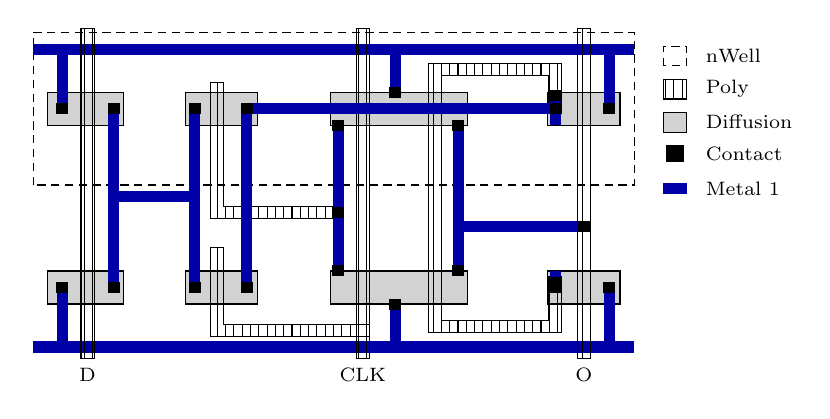
\begin{tikzpicture}[x=.92cm,y=.84cm,font=\scriptsize,
  act/.style={fill=gray!35,draw=black,thin},
  poly/.style={draw=black,fill=white,pattern=vertical lines,pattern color=black},
  metal/.style={draw=blue!65!black,line width=4pt},
  ct/.style={fill=black,draw=black}]
% Printed n-well, metal rails and four diffusion islands in each row.
\draw[densely dashed](-.05,2.65)rectangle(8.25,4.95);
\draw[metal](-.05,4.7)--(8.25,4.7);
\draw[metal](-.05,.2)--(8.25,.2);
\foreach \y in {3.8,1.1}{
 \path[act](.15,{\y-.25})rectangle(1.2,{\y+.25});
 \path[act](2.05,{\y-.25})rectangle(3.05,{\y+.25});
 \path[act](4.05,{\y-.25})rectangle(5.95,{\y+.25});
 \path[act](7.05,{\y-.25})rectangle(8.05,{\y+.25});}
% Continuous external D/CLK/O gates; the TG clock gate is split.
\foreach \x in {.7,4.5,7.55}{\path[poly]({\x-.09},.03)rectangle({\x+.09},5.02);}
\path[poly](2.4,2.14)--(4.16,2.14)--(4.16,2.32)--(2.58,2.32)--(2.58,4.2)--(2.4,4.2)--cycle;
\path[poly](2.4,.36)--(4.59,.36)--(4.59,.54)--(2.58,.54)--(2.58,1.7)--(2.4,1.7)--cycle;
% Continuous storage-inverter poly, with both U-return arms.
\path[poly](5.41,.42)--(7.24,.42)--(7.24,1.27)--(7.06,1.27)--(7.06,.60)--(5.59,.60)--(5.59,4.30)--(7.06,4.30)--(7.06,3.90)--(7.24,3.90)--(7.24,4.48)--(5.41,4.48)--cycle;
% Supply contacts (a metal crossing alone is not an electrical contact).
\draw[metal](.35,3.8)--(.35,4.7);
\draw[metal](.35,1.1)--(.35,.2);
\draw[metal](4.95,4.05)--(4.95,4.7);
\draw[metal](4.95,.85)--(4.95,.2);
\draw[metal](7.9,3.8)--(7.9,4.7);
\draw[metal](7.9,1.1)--(7.9,.2);
% dbar: first-inverter drains and left TG terminals.
\draw[metal](1.06,3.8)--(1.06,1.1);
\draw[metal](1.06,2.48)--(2.18,2.48);
\draw[metal](2.18,3.8)--(2.18,1.1);
% u: TG right terminals, final-inverter drains and U-poly contacts.
\draw[metal](2.9,3.8)--(2.9,1.1);
\draw[metal](2.9,3.8)--(7.16,3.8);
% Separate final-drain stubs: their common u connection is via the U-poly.
% A vertical Metal1 through the middle gap would wrongly short the O route.
\draw[metal](7.16,4.0)--(7.16,3.55);
\draw[metal](7.16,1.35)--(7.16,1.1);
% CLKB: CLK inverter drains return to the UPPER TG poly only.
\draw[metal](4.16,3.55)--(4.16,1.35);
% O: storage-inverter drains join the final O poly at one contact.
\draw[metal](5.82,3.55)--(5.82,1.35);
\draw[metal](5.82,2.02)--(7.55,2.02);
\foreach \x/\y in {.35/3.8,.35/1.1,1.06/3.8,1.06/1.1,2.18/3.8,2.18/1.1,2.9/3.8,2.9/1.1,4.16/3.55,4.16/1.35,4.95/4.05,4.95/.85,5.82/3.55,5.82/1.35,7.16/3.8,7.16/1.1,7.9/3.8,7.9/1.1,4.16/2.23,7.16/4.0,7.16/1.18,7.55/2.02}{
 \path[ct]({\x-.075},{\y-.075})rectangle({\x+.075},{\y+.075});}
\node[below]at(.7,.02){D};\node[below]at(4.5,.02){CLK};\node[below]at(7.55,.02){O};
\draw[densely dashed](8.65,4.45)rectangle(8.97,4.75);\node[right]at(9.10,4.6){nWell};
\path[poly](8.65,3.95)rectangle(8.97,4.25);\node[right]at(9.10,4.1){Poly};
\path[act](8.65,3.45)rectangle(8.97,3.75);\node[right]at(9.10,3.6){Diffusion};
\path[ct](8.69,3.0)rectangle(8.93,3.24);\node[right]at(9.10,3.12){Contact};
\draw[metal](8.65,2.6)--(8.97,2.6);\node[right]at(9.10,2.6){Metal 1};
\end{tikzpicture}}

\newcommand{\SolutionLayout}{%
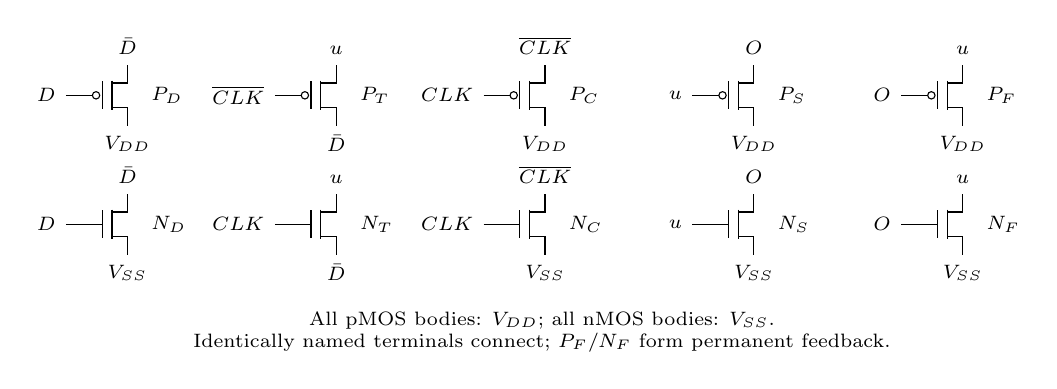
\begin{tikzpicture}[scale=.78,font=\scriptsize]
% Every MOS is explicit. Identically named terminals are joined.
\mos{0}{1}{D}{1}\node[right]at(.48,1){$P_D$};\node[above]at(.25,1.5){$\bar D$};\node[below]at(.25,.5){$V_{DD}$};
\mos{3.4}{1}{\overline{CLK}}{1}\node[right]at(3.88,1){$P_T$};\node[above]at(3.65,1.5){$u$};\node[below]at(3.65,.5){$\bar D$};
\mos{6.8}{1}{CLK}{1}\node[right]at(7.28,1){$P_C$};\node[above]at(7.05,1.5){$\overline{CLK}$};\node[below]at(7.05,.5){$V_{DD}$};
\mos{10.2}{1}{u}{1}\node[right]at(10.68,1){$P_S$};\node[above]at(10.45,1.5){$O$};\node[below]at(10.45,.5){$V_{DD}$};
\mos{13.6}{1}{O}{1}\node[right]at(14.08,1){$P_F$};\node[above]at(13.85,1.5){$u$};\node[below]at(13.85,.5){$V_{DD}$};
\mos{0}{-1.1}{D}{0}\node[right]at(.48,-1.1){$N_D$};\node[above]at(.25,-.6){$\bar D$};\node[below]at(.25,-1.6){$V_{SS}$};
\mos{3.4}{-1.1}{CLK}{0}\node[right]at(3.88,-1.1){$N_T$};\node[above]at(3.65,-.6){$u$};\node[below]at(3.65,-1.6){$\bar D$};
\mos{6.8}{-1.1}{CLK}{0}\node[right]at(7.28,-1.1){$N_C$};\node[above]at(7.05,-.6){$\overline{CLK}$};\node[below]at(7.05,-1.6){$V_{SS}$};
\mos{10.2}{-1.1}{u}{0}\node[right]at(10.68,-1.1){$N_S$};\node[above]at(10.45,-.6){$O$};\node[below]at(10.45,-1.6){$V_{SS}$};
\mos{13.6}{-1.1}{O}{0}\node[right]at(14.08,-1.1){$N_F$};\node[above]at(13.85,-.6){$u$};\node[below]at(13.85,-1.6){$V_{SS}$};
\node[align=center]at(7,-2.85){All pMOS bodies: $V_{DD}$; all nMOS bodies: $V_{SS}$.\\Identically named terminals connect; $P_F/N_F$ form permanent feedback.};
\end{tikzpicture}}

\begin{document}
\begin{center}{\large\bfseries Fall 2007 Final -- Corrected, Independently Checked Solutions}\end{center}
\textbf{Scope.} All seven questions and their original 105\% weights are retained. Two ungraded student sources are comparison material only. Logic follows the printed connections; missing transistor ratios, clock duty cycle and minimum timing data are explicitly qualified.

\textbf{1. Short answers.}
\begin{enumerate}[label=(\alph*),leftmargin=7mm,itemsep=5pt]
\item Define specifications and architecture; create transistor schematics; simulate and size the circuit; draw layout; run DRC and LVS; extract parasitics; perform post-layout simulation and signoff; prepare the verified mask database. Student ``pre-simulation, layout, DRC, LVS, post-simulation'' is a useful subset but omits specification, circuit creation and parasitic extraction.
\item Use a common cell height, and align VDD/VSS rails for legal abutment. Variable cell width is normal, but is not a replacement for the height/rail rules. All process design rules still apply.
\item Charge sharing can corrupt a dynamic level; directly cascading same-phase dynamic gates can cause an erroneous irreversible downstream discharge. Leakage and noise are additional problems.
\item Ordinary N-domino cascades implement noninverting functions, and evaluation inputs must be monotonic low-to-high. A required output buffer is a structural feature; explain its role rather than treating it as an arbitrary restriction.
\item Core-limited die dimensions are determined mainly by logic and routing area; pad-limited die dimensions are determined mainly by pad count and perimeter/pitch requirements.
\end{enumerate}

\textbf{2. XNOR, with ratioed-level assumptions.}
\begin{center}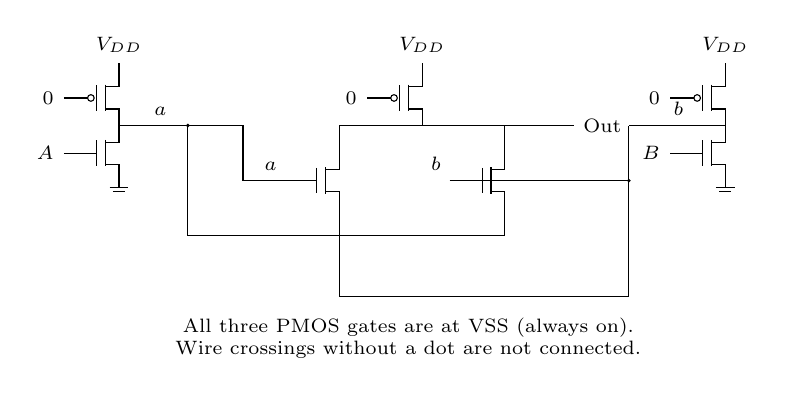
\begin{tikzpicture}[scale=.7,font=\scriptsize]
\mos{0}{5}{0}{1}\rail{.25}{5.5}{V_{DD}}\mos{0}{4}{A}{0}\ground{.25}{3.5}\node[above]at(1,4.5){$a$};\draw(.25,4.5)--(1.5,4.5);
\mos{11}{5}{0}{1}\rail{11.25}{5.5}{V_{DD}}\mos{11}{4}{B}{0}\ground{11.25}{3.5}\node[above]at(10.4,4.5){$b$};\draw(11.25,4.5)--(9.5,4.5);
\mos{5.5}{5}{0}{1}\rail{5.75}{5.5}{V_{DD}}\draw(4.25,4.5)--(8.5,4.5)node[right]{Out};\mos{4}{3.5}{\phantom{a}}{0}\mos{7}{3.5}{\phantom{b}}{0}\draw(4.25,4)--(4.25,4.5);\draw(7.25,4)--(7.25,4.5);\node[above]at(3,3.5){$a$};\node[above]at(6,3.5){$b$};
\draw(1.5,4.5)--(2.5,4.5)--(2.5,3.5)--(3.25,3.5);\draw(1.5,4.5)--(1.5,2.5)--(7.25,2.5)--(7.25,3);\fill(1.5,4.5)circle(1pt);
\draw(4.25,3)--(4.25,1.4)--(9.5,1.4)--(9.5,4.5);\draw(9.5,3.5)--(6.25,3.5);\fill(9.5,3.5)circle(1pt);
\node[align=center]at(5.5,.65){All three PMOS gates are at VSS (always on).\\Wire crossings without a dot are not connected.};\end{tikzpicture}\end{center}
The outer two device pairs are pseudo-NMOS inverters: their PMOS gates are 0 and always on. If their pull-downs are sufficiently stronger than their loads, $a=\bar A$, $b=\bar B$. The output PMOS also is always on. One output NMOS has gate a and channel Out--b; the other has gate b and channel Out--a.
\begin{center}\begin{tabular}{cccccl}\toprule
A&B&a&b&Out&Reason\\\midrule
0&0&1&1&1&Both pass paths end at high nodes.\\
0&1&1&0&0&Gate a enables the path to low b.\\
1&0&0&1&0&Gate b enables the path to low a.\\
1&1&0&0&1&Both output NMOS are off; PMOS pulls high.\\\bottomrule\end{tabular}\end{center}
\[\boxed{\mathrm{Out}=AB+\bar A\bar B=\overline{A\oplus B}.}\]
The unequal-input low involves contention with always-on PMOS and the associated outer inverter load. The exact low voltage and static power require device strengths and supply data that are absent. Thus XNOR is the intended Boolean function, conditional on valid ratioed low levels; this is not complementary, ratio-independent static CMOS. Both students' XNOR tables are accepted after checking the actual cross-connected channel terminals.

\newpage\textbf{3. Contact-extracted CMOS schematic.}
\begin{center}\SolutionLayout\end{center}
The five active/poly crossing columns contain ten MOS: the two internal poly routes also cross upper and lower active regions. They are four CMOS inverters and one transmission gate. Repeated labelled channel/gate nets in the complete extraction refer to the same wire. The contact audit and literal MOS netlist are included beside this document.
\[
\bar D=\operatorname{INV}(D),\quad \overline{\mathrm{CLK}}=\operatorname{INV}(\mathrm{CLK}),\quad
O=\operatorname{INV}(u),\quad u=\operatorname{INV}(O)\quad\hbox{through fixed feedback.}
\]
The transmission gate joins $\bar D$ and u, with its PMOS gate at $\overline{\mathrm{CLK}}$ and NMOS gate at CLK. Its two poly gates are physically separate; the drawn continuous CLK column belongs to the clock inverter. The rightmost O-labelled poly is an inverter input, connected to the adjacent storage inverter's output through a metal/poly contact; its drain return is u.

For CLK=0, the transmission gate is off and the cross-coupled inverter loop stores O. For CLK=1, the input path attempts to drive $u=\bar D$, giving the noninverting transparent relation $O=D$. The feedback inverter is \emph{not} disconnected during writing. If the new D differs from the old O, it opposes the input driver. Successful overwrite therefore requires sufficient input-inverter/transmission-gate drive relative to that fixed feedback; the source supplies no widths. The extracted topology is certain, while unconditional writeability is not proven. A conventional latch with a second feedback transmission gate would alter the printed layout. The student sketches agree on the intended latch class, but cannot establish omitted strength assumptions. This strength condition agrees with the fixed-feedback latch discussion in \href{https://www.ee.ncu.edu.tw/jfli/public_html/VLSI/lecture/ch07.pdf}{NCU course Chapter 7, slide 9}; that reference does not replace the source contact trace.

\newpage\textbf{4. NP-domino full adder and retention.}
\begin{center}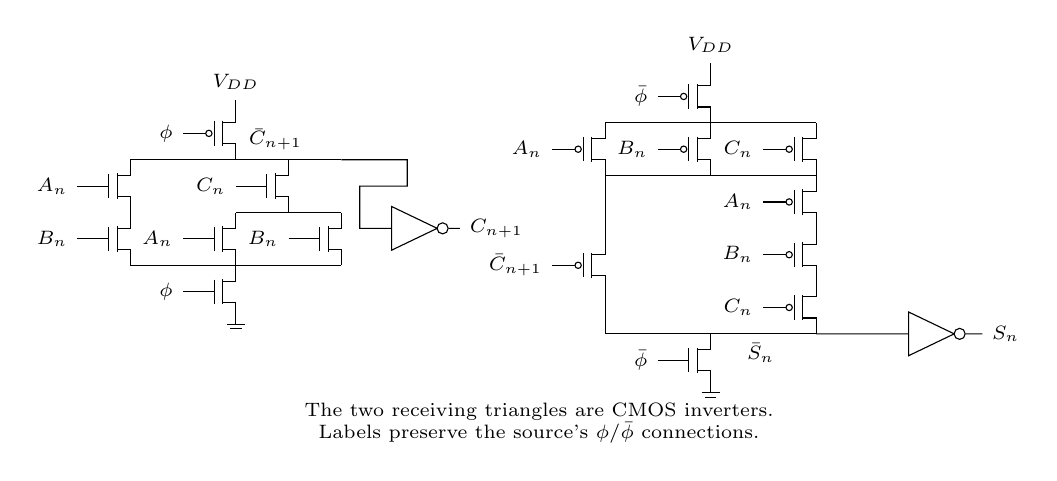
\begin{tikzpicture}[scale=.67,font=\scriptsize]
\mos{2}{5.8}{\phi}{1}\rail{2.25}{6.3}{V_{DD}}\draw(.25,5.3)--(4.25,5.3);\node[above]at(3,5.3){$\bar C_{n+1}$};\mos{0}{4.8}{A_n}{0}\mos{0}{3.8}{B_n}{0}\mos{3}{4.8}{C_n}{0}\draw(3.25,4.3)--(4.25,4.3);\mos{2}{3.8}{A_n}{0}\mos{4}{3.8}{B_n}{0}\draw(2.25,4.3)--(3.25,4.3);\draw(.25,3.3)--(4.25,3.3);\mos{2}{2.8}{\phi}{0}\ground{2.25}{2.3}
\node[not gate US,draw,minimum width=.65cm](ci)at(5.5,4){};\draw(4.25,5.3)--(5.5,5.3)--(5.5,4.8)--(4.6,4.8)--(4.6,4)--(ci.input);\draw(ci.output)--(6.5,4)node[right]{$C_{n+1}$};
\mos{11}{6.5}{\bar\phi}{1}\rail{11.25}{7}{V_{DD}}\draw(9.25,6)--(13.25,6);\mos{9}{5.5}{A_n}{1}\mos{11}{5.5}{B_n}{1}\mos{13}{5.5}{C_n}{1}\draw(9.25,5)--(13.25,5);
\mos{9}{3.3}{\bar C_{n+1}}{1}\draw(9.25,3.8)--(9.25,5);\draw(9.25,2.8)--(9.25,2)--(13.25,2);\mos{13}{4.5}{A_n}{1}\mos{13}{3.5}{B_n}{1}\mos{13}{2.5}{C_n}{1}\mos{11}{1.5}{\bar\phi}{0}\ground{11.25}{1}\node[below]at(12.2,2){$\bar S_n$};\node[not gate US,draw,minimum width=.65cm](si)at(15.3,2){};\draw(13.25,2)--(si.input);\draw(si.output)--(16.4,2)node[right]{$S_n$};
\node[align=center]at(8,.3){The two receiving triangles are CMOS inverters.\\Labels preserve the source's $\phi/\bar\phi$ connections.};\end{tikzpicture}\end{center}
\textbf{(a)} This is NP-domino logic: an N-type dynamic carry network feeds a P-type dynamic sum network, with CMOS output inverters. The N network evaluates when $\phi=1$; the P network also evaluates then because its header/pre-discharge controls are $\bar\phi$.

\textbf{(b)} Define $M=A_nB_n+C_n(A_n+B_n)$. During precharge $\phi=0$, $\bar C_{n+1}=1$ and $\bar S_n=0$, so the buffered outputs are carry 0 and sum 1. These are precharge values, not valid full-adder results. During evaluation $\phi=1$,
\[\bar C_{n+1}=\bar M,\qquad C_{n+1}=M.\]
The P sum network has its three input PMOS in parallel \emph{before} the two alternative branches. Its pull-up condition is
\[
\begin{aligned}
\bar S_n&=(\bar A_n+\bar B_n+\bar C_n)\bigl(\overline{\bar C_{n+1}}+\bar A_n\bar B_n\bar C_n\bigr)
=\overline{A_n\oplus B_n\oplus C_n},\\
S_n&=A_n\oplus B_n\oplus C_n.
\end{aligned}
\]
The double bar on $\bar C_{n+1}$ is the carry M, not a second independent carry signal. The outputs become valid after the evaluation paths settle. The student PDF's phase table treats the P-stage evaluation incorrectly; the separate student JPEG's full-adder expressions are consistent after this network check.

\textbf{(c)} At $\bar C_{n+1}$, three drains meet (precharge P, top A N, top C N), and three receiving gates load the node (two carry-inverter gates plus the P-network carry-input gate). Thus
\[C_{\bar C}=3C_d+3C_g=3(0.2)+3(1)=3.6\ \mathrm{fF}.\]
At $\bar S_n$, three drains meet (carry-input P, bottom serial C P, pre-discharge N), and two sum-inverter gates load it:
\[C_{\bar S}=3C_d+2C_g=3(0.2)+2(1)=2.6\ \mathrm{fF}.\]
With worst adverse leakage 1 nA and allowed deviation 0.9 V from the stored rail, charge conservation gives
\[t_{hold,carry}=\frac{3.6\mathrm{fF}\cdot0.9\mathrm V}{1\mathrm{nA}}=3.24\ \mu\mathrm s,
\quad t_{hold,sum}=2.34\ \mu\mathrm s.\]
The smaller sum capacitance governs. Therefore the principal result is
\[\boxed{t_{evaluation}<2.34\ \mu\mathrm s.}\]
If D is the fraction of a full clock cycle spent evaluating, $t_{evaluation}=D/f$, so
\[\boxed{f>\frac{D}{2.34\,\mu\mathrm s}.}\]
For an \emph{explicitly assumed} 50\% evaluation duty, this is about 213.7 kHz. Treating an entire period as the leakage interval gives 427.4 kHz, but that is a different conservative convention, not a duty cycle established by the printed problem. The separate student JPEG correctly counts 2.6 fF but uses the full-period convention; the student PDF considers only the nonlimiting carry node. Neither ungraded answer supplies a missing clock-duty premise. Equality reaches the inverter threshold with zero noise margin.

\newpage\textbf{5. Correct output polarity in all three logic styles.}
Let $g=A(B+C)+DE$, $f=\bar g=(\bar A+\bar B\bar C)(\bar D+\bar E)$.
\textbf{(1) Domino core plus explicit output inversion.} A standard N-domino core with g's NMOS network has precharge node z=$\bar g$ and buffered, monotonic output g. To produce the requested negative function at the primary output, add a \emph{second} static inverter, giving 11 MOS:
\begin{center}\begin{tikzpicture}[x=.8cm,y=.82cm,font=\scriptsize]
\mos{0}{0.0}{\phi}{1}\node[right]at(0.45,0.45){$\mathrm{Ppre}$};\node[above]at(0.25,0.5){$V_{DD}$};\node[below]at(0.25,-0.5){$z$};
\mos{5}{0.0}{A}{0}\node[right]at(5.45,0.45){$\mathrm{NA}$};\node[above]at(5.25,0.5){$z$};\node[below]at(5.25,-0.5){$u$};
\mos{10}{0.0}{B}{0}\node[right]at(10.45,0.45){$\mathrm{NB}$};\node[above]at(10.25,0.5){$u$};\node[below]at(10.25,-0.5){$foot$};
\mos{0}{-2.25}{C}{0}\node[right]at(0.45,-1.8){$\mathrm{NC}$};\node[above]at(0.25,-1.75){$u$};\node[below]at(0.25,-2.75){$foot$};
\mos{5}{-2.25}{D}{0}\node[right]at(5.45,-1.8){$\mathrm{ND}$};\node[above]at(5.25,-1.75){$z$};\node[below]at(5.25,-2.75){$v$};
\mos{10}{-2.25}{E}{0}\node[right]at(10.45,-1.8){$\mathrm{NE}$};\node[above]at(10.25,-1.75){$v$};\node[below]at(10.25,-2.75){$foot$};
\mos{0}{-4.5}{\phi}{0}\node[right]at(0.45,-4.05){$\mathrm{Nfoot}$};\node[above]at(0.25,-4.0){$foot$};\node[below]at(0.25,-5.0){$0$};
\mos{5}{-4.5}{z}{1}\node[right]at(5.45,-4.05){$\mathrm{Pi1}$};\node[above]at(5.25,-4.0){$V_{DD}$};\node[below]at(5.25,-5.0){$g$};
\mos{10}{-4.5}{z}{0}\node[right]at(10.45,-4.05){$\mathrm{Ni1}$};\node[above]at(10.25,-4.0){$g$};\node[below]at(10.25,-5.0){$0$};
\mos{0}{-6.75}{g}{1}\node[right]at(0.45,-6.3){$\mathrm{Pi2}$};\node[above]at(0.25,-6.25){$V_{DD}$};\node[below]at(0.25,-7.25){$f$};
\mos{5}{-6.75}{g}{0}\node[right]at(5.45,-6.3){$\mathrm{Ni2}$};\node[above]at(5.25,-6.25){$f$};\node[below]at(5.25,-7.25){$0$};
\end{tikzpicture}\end{center}
Only the internal g signal is an ordinary N-domino cascading signal; the final f is a static inversion and is not a monotonic N-domino cascade output. A strict single-domino-stage alternative realizes f's 5-device NMOS network using complementary inputs, then one inverter (9-device core plus 10 MOS to generate missing complements). In that alternative, the complemented evaluation inputs must obey the monotonicity requirement. Either explicit construction produces f. The student's g-network followed by only one inverter produces g, not f, so that sketch is corrected.

\newpage\textbf{(2) Fully differential logic.} The two NMOS networks realize g and f, respectively. Cross-coupled PMOS loads directly sense the opposite full-swing output; no reference-voltage clamps are used. The 12-device core is:
\begin{center}\begin{tikzpicture}[x=.8cm,y=.82cm,font=\scriptsize]
\mos{0}{0.0}{fb}{1}\node[right]at(0.45,0.45){$\mathrm{Pz}$};\node[above]at(0.25,0.5){$V_{DD}$};\node[below]at(0.25,-0.5){$z$};
\mos{5}{0.0}{z}{1}\node[right]at(5.45,0.45){$\mathrm{Pfb}$};\node[above]at(5.25,0.5){$V_{DD}$};\node[below]at(5.25,-0.5){$fb$};
\mos{10}{0.0}{A}{0}\node[right]at(10.45,0.45){$\mathrm{NA}$};\node[above]at(10.25,0.5){$z$};\node[below]at(10.25,-0.5){$u$};
\mos{0}{-2.25}{B}{0}\node[right]at(0.45,-1.8){$\mathrm{NB}$};\node[above]at(0.25,-1.75){$u$};\node[below]at(0.25,-2.75){$0$};
\mos{5}{-2.25}{C}{0}\node[right]at(5.45,-1.8){$\mathrm{NC}$};\node[above]at(5.25,-1.75){$u$};\node[below]at(5.25,-2.75){$0$};
\mos{10}{-2.25}{D}{0}\node[right]at(10.45,-1.8){$\mathrm{ND}$};\node[above]at(10.25,-1.75){$z$};\node[below]at(10.25,-2.75){$v$};
\mos{0}{-4.5}{E}{0}\node[right]at(0.45,-4.05){$\mathrm{NE}$};\node[above]at(0.25,-4.0){$v$};\node[below]at(0.25,-5.0){$0$};
\mos{5}{-4.5}{\bar A}{0}\node[right]at(5.45,-4.05){$\mathrm{Na}$};\node[above]at(5.25,-4.0){$fb$};\node[below]at(5.25,-5.0){$w$};
\mos{10}{-4.5}{\bar B}{0}\node[right]at(10.45,-4.05){$\mathrm{Nb}$};\node[above]at(10.25,-4.0){$fb$};\node[below]at(10.25,-5.0){$t$};
\mos{0}{-6.75}{\bar C}{0}\node[right]at(0.45,-6.3){$\mathrm{Nc}$};\node[above]at(0.25,-6.25){$t$};\node[below]at(0.25,-7.25){$w$};
\mos{5}{-6.75}{\bar D}{0}\node[right]at(5.45,-6.3){$\mathrm{Nd}$};\node[above]at(5.25,-6.25){$w$};\node[below]at(5.25,-7.25){$0$};
\mos{10}{-6.75}{\bar E}{0}\node[right]at(10.45,-6.3){$\mathrm{Ne}$};\node[above]at(10.25,-6.25){$w$};\node[below]at(10.25,-7.25){$0$};
\end{tikzpicture}\end{center}
Here z is f, and fb is $\bar f=g$. If complementary inputs are not externally available, add five CMOS inverters (10 MOS), total 22. For every binary ABCDE exactly one pull-down conducts, so the two outputs are complementary. The student's differential topology is accepted with these explicit net/output labels and input-complement generators.

\textbf{(3) Static CMOS.} Use the g pull-down and its complementary f pull-up (10 MOS):
\begin{center}\begin{tikzpicture}[x=.8cm,y=.82cm,font=\scriptsize]
\mos{0}{0.0}{A}{0}\node[right]at(0.45,0.45){$\mathrm{NA}$};\node[above]at(0.25,0.5){$z$};\node[below]at(0.25,-0.5){$u$};
\mos{5}{0.0}{B}{0}\node[right]at(5.45,0.45){$\mathrm{NB}$};\node[above]at(5.25,0.5){$u$};\node[below]at(5.25,-0.5){$0$};
\mos{10}{0.0}{C}{0}\node[right]at(10.45,0.45){$\mathrm{NC}$};\node[above]at(10.25,0.5){$u$};\node[below]at(10.25,-0.5){$0$};
\mos{0}{-2.25}{D}{0}\node[right]at(0.45,-1.8){$\mathrm{ND}$};\node[above]at(0.25,-1.75){$z$};\node[below]at(0.25,-2.75){$v$};
\mos{5}{-2.25}{E}{0}\node[right]at(5.45,-1.8){$\mathrm{NE}$};\node[above]at(5.25,-1.75){$v$};\node[below]at(5.25,-2.75){$0$};
\mos{10}{-2.25}{A}{1}\node[right]at(10.45,-1.8){$\mathrm{PA}$};\node[above]at(10.25,-1.75){$V_{DD}$};\node[below]at(10.25,-2.75){$p1$};
\mos{0}{-4.5}{B}{1}\node[right]at(0.45,-4.05){$\mathrm{PB}$};\node[above]at(0.25,-4.0){$V_{DD}$};\node[below]at(0.25,-5.0){$p2$};
\mos{5}{-4.5}{C}{1}\node[right]at(5.45,-4.05){$\mathrm{PC}$};\node[above]at(5.25,-4.0){$p2$};\node[below]at(5.25,-5.0){$p1$};
\mos{10}{-4.5}{D}{1}\node[right]at(10.45,-4.05){$\mathrm{PD}$};\node[above]at(10.25,-4.0){$p1$};\node[below]at(10.25,-5.0){$z$};
\mos{0}{-6.75}{E}{1}\node[right]at(0.45,-6.3){$\mathrm{PE}$};\node[above]at(0.25,-6.25){$p1$};\node[below]at(0.25,-7.25){$z$};
\end{tikzpicture}\end{center}
The output z is the requested f. Five pull-up gates use the original, uncomplemented input variables; the PMOS on conditions supply the logical complements. External input inverters are unnecessary here.

\newpage\textbf{6. A dynamic falling-edge D register.}
\begin{center}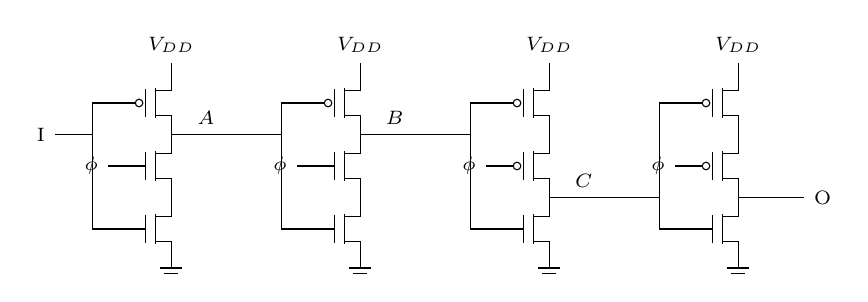
\begin{tikzpicture}[scale=.8,font=\scriptsize]
\mos{0}{4}{\phantom{I}}{1}\rail{0.25}{4.5}{V_{DD}}\mos{0}{3}{\phi}{0}\mos{0}{2}{\phantom{I}}{0}\ground{0.25}{1.5}
\node[above]at(0.8,3.5){$ A $};
\draw(-1,2)--(-1,4)--(-.75,4);\draw(-1,2)--(-.75,2);\draw(-1.6,3.5)node[left]{I}--(-1,3.5);
\mos{3}{4}{\phantom{A}}{1}\rail{3.25}{4.5}{V_{DD}}\mos{3}{3}{\phi}{0}\mos{3}{2}{\phantom{A}}{0}\ground{3.25}{1.5}
\node[above]at(3.8,3.5){$ B $};
\draw(0.25,3.5)--(2,3.5)--(2,4)--(2.25,4);\draw(2,3.5)--(2,2)--(2.25,2);
\mos{6}{4}{\phantom{B}}{1}\rail{6.25}{4.5}{V_{DD}}\mos{6}{3}{\phi}{1}\mos{6}{2}{\phantom{B}}{0}\ground{6.25}{1.5}
\node[above]at(6.8,2.5){$C$};
\draw(3.25,3.5)--(5,3.5)--(5,4)--(5.25,4);\draw(5,3.5)--(5,2)--(5.25,2);
\mos{9}{4}{\phantom{C}}{1}\rail{9.25}{4.5}{V_{DD}}\mos{9}{3}{\phi}{1}\mos{9}{2}{\phantom{C}}{0}\ground{9.25}{1.5}
\draw(6.25,2.5)--(8,2.5)--(8,4)--(8.25,4);\draw(8,2.5)--(8,2)--(8.25,2);
\draw(9.25,2.5)--(10.3,2.5)node[right]{O};\end{tikzpicture}\end{center}
There are four 3-transistor split inverters, 12 MOS total. In the first pair, each PMOS is input-controlled and its NMOS path includes a clock NMOS; in the second pair, the PMOS path includes a clock PMOS and the NMOS is input-controlled.
\begin{center}\begin{tabular}{cllll}\toprule
Clock phase&A&B&C&O\\\midrule
$\phi=1$&$\bar I$&I&Can be forced low&Held from preceding low phase\\
Falling edge&Master closes&Stored I&$\bar B$&B (new sampled I)\\
$\phi=0$&May force high&Stored&$\bar B$&B\\
Rising edge&Master opens&Tracks new I&Slave closes&Previous sampled value held\\\bottomrule\end{tabular}\end{center}
While $\phi=1$, the first two inversions give B=I. After $\phi$ falls, the first pair preserves B: a later I change may force A high, but the second pull-up then switches off rather than corrupting B. The second pair is enabled for $\phi=0$, giving C=$\bar B$ and O=B. When $\phi$ rises, its P clock devices turn off and the two-node storage pattern protects O even as B changes. Thus O samples I on the \textbf{falling edge}, with an overall even number of inversions.
Several nodes retain charge dynamically; this is not a static cross-coupled latch with indefinite retention. Clock pulse widths, setup/hold and leakage limit the practical operation. Student JPEG's falling-edge interpretation agrees. Student PDF's $\phi=1,I=0,B=1$ table entry does not: A=1 enables the second NMOS discharge, so B must be 0.

\textbf{7. Setup-limited clock period and the missing minimum delays.}
At the printed common clock (zero skew), setup requires
\[T\geq t_{pcq}+t_{pd}+t_{setup}=2+15+3=20\ \mathrm{ns}.
\quad\boxed{T_{min,setup}=20\ \mathrm{ns},\quad f_{max,setup}=50\ \mathrm{MHz}.}\]
The student setup sum is correct. Hold separately requires $t_{ccq}+t_{cd}\geq1$ ns. The problem gives propagation delays, not distinct minimum clock-to-Q/combinational delays, so setup alone does not prove hold. In the simple fixed-delay interpretation (2 ns and 15 ns also minimum delays), the hold margin is $2+15-1=16$ ns and the 20 ns clock is valid. Otherwise minimum-delay characterization is needed; increasing clock period does not repair a hold violation.
\small All switch truth tables, full-adder states, dynamic-register phase events, capacitance counts and timing/retention calculations are independently checked by verify.py. The figures remain editable and retain the printed connections.\end{document}
